% =============================================================================
% COPYRIGHT AND DISCLAIMER
% =============================================================================
% This file is provided as a convenience template for competition participants.
% By using it, you accept full responsibility for compliance with all applicable
% copyright, licensing, and usage rules of the Association for Computing
% Machinery (ACM) and of any LaTeX packages you load (including, without
% limitation, the "acmart" document class and related ACM materials).
%
% Consult ACM's official publication, template, and copyright policies before
% using this setup for any purpose other than this competition. Do not assume
% that this template may be reused, redistributed, or submitted elsewhere
% without independently verifying ACM's current rules.
%
% Use of the "acmart" class, the "sigconf" option, or ACM-style formatting in
% this template does NOT mean that this report, this competition, its organizers,
% or any resulting PDF is sponsored, endorsed, affiliated with, or published by
% ACM. ACM trademarks and branding remain the property of ACM.
%
% Template packages live in preamble.tex.
% Citations live in main.bib. Edit this file with your paper content.
% =============================================================================

\documentclass[sigconf]{acmart}
\input{preamble}
\newcommand{\TBD}[1]{\textcolor{red}{#1}}   % numbers still to be filled in (none must remain at the end)

% Guide styling: \guideStyletrue = show gray italic hints; \guideStylefalse = omit them
% \guideStyletrue
\guideStylefalse

\begin{document}

\title{Limb-Flattened Inputs, a Pretrained ResNet-50 U-Net and PQ-Tuned Instance Formation for Solar Filament Segmentation}
\subtitle{A Solution to the Solar Filament Segmentation Challenge 2026} % DO NOT CHANGE


\author{Amoli Kakkar}
\affiliation{%
  \institution{Independent researcher}
  \state{Rajasthan}
  \country{India}
}
\email{amolikakkar@gmail.com}

\begin{abstract}
    This report describes our solution to the Solar Filament Segmentation Challenge~2026, a Kaggle competition on automatic segmentation of solar filaments in GONG H-$\alpha$ observations. Each image is first corrected for limb darkening and large-scale brightness gradients, so that the quiet Sun has a uniform intensity of about one. A U-Net with an ImageNet-pretrained ResNet-50 encoder then predicts a filament probability map, which is turned into filament instances by a threshold, a size filter and distance-based fragment linking, all chosen to maximise the organisers' dataset-level Panoptic Quality (PQ). On 106 held-out training images (168 annotator versions) the model reaches PQ~0.419 (95\% bootstrap interval 0.399--0.439), compared with 0.411 for the same design with a ResNet-34 encoder (public leaderboard 0.33), 0.338 for a compact U-Net trained on a laptop CPU and 0.262 for a training-free classical detector. Code, weights and a notebook that reproduces the submission on a CPU without retraining are public.
\end{abstract}

\maketitle

\ifguideStyle
\noindent{\color{gray!65}\itshape
Guide mode is on.}
\par\medskip
\fi


% ==================================== %
%              INTRODUCTION            %
% ==================================== %
\section{Introduction}
    This report goes over the details of our submitted solution to the Solar Filament Segmentation Challenge~2026 \cite{filament-segmentation-2026}. The challenge, launched on July~10,~2026, is organized by the Earth-Space AI Research (ESAIR) Lab\footnote{\href{https://www.esairlab.com/home}{www.esairlab.com/}}. This challenge utilizes the MAGFiLO dataset for evaluation of the segmentation algorithms \cite{ahmadzadeh2024dataset}. Because PQ only counts a prediction when its IoU with an annotated filament exceeds 0.5 \cite{kirillov2019panoptic}, a solution must find each filament, outline it well, and keep it in one piece without merging it with its neighbours. Our pipeline treats these three needs separately: (i) a physics-motivated flattening step that removes the brightness variation that is not caused by filaments; (ii) a semantic U-Net \cite{ronneberger2015unet} that only has to say ``filament or not''; and (iii) an instance step whose parameters are tuned directly for the competition metric. We also report two lighter baselines that share steps (i) and (iii): a training-free classical detector and a compact U-Net trained on a laptop CPU.


% ==================================== %
%              METHODOLOGY             %
% ==================================== %
\section{Methodology}\label{sec:methodology}

\begin{figure*}[t]
  \centering
  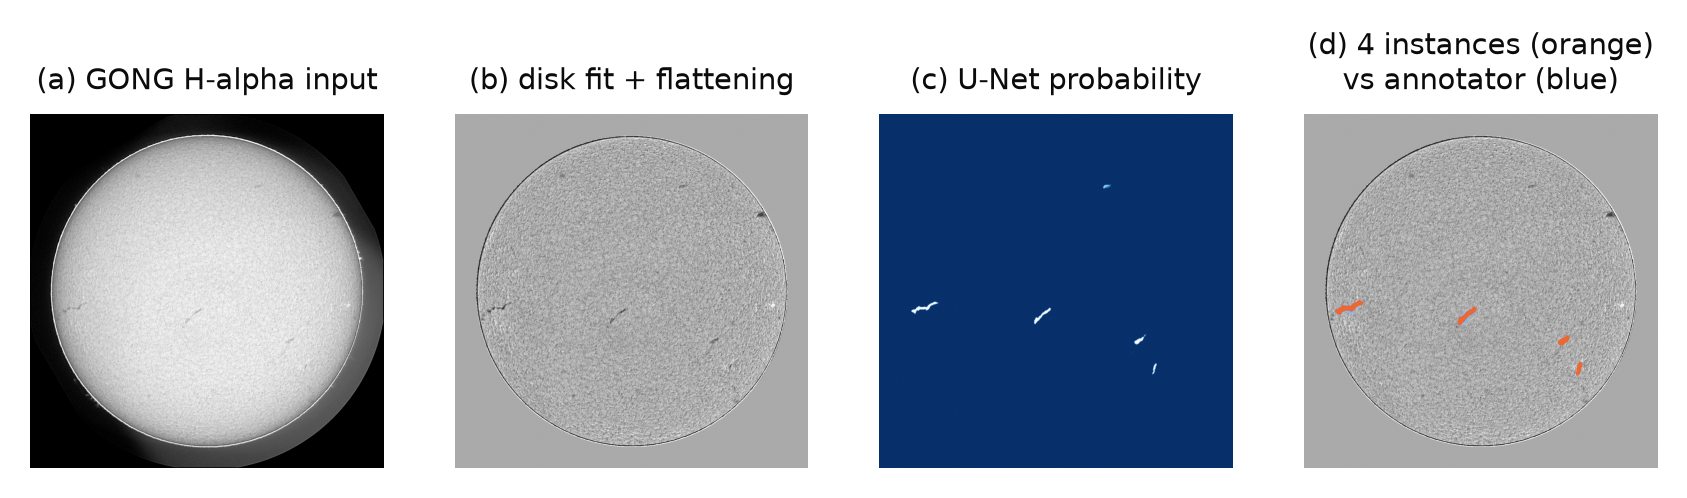
\includegraphics[width=\textwidth]{fig_pipeline.png}
  \caption{End-to-end pipeline on a validation image. (a) Raw 2048$\times$2048 GONG H-$\alpha$ image. (b) Disk fit and flattening (quiet Sun $\approx 1$). (c) U-Net probability (1024\,px, flip test-time augmentation). (d) Threshold and size filter give the predicted instances (orange), shown against one annotator's polygons (blue). Each instance is then RLE-encoded for the submission.}
  \label{fig:pipeline}
\end{figure*}

\subsection{Data and sampling}
The training set has 707 image files with 1,154 annotation entries (several annotators per image) and 8,199 filament polygons; the test set has 180 images. We hold out 15\% of the image \emph{files} (random seed 0): 106 files with 168 annotator entries form the validation set and 601 files with 986 entries the training set. Splitting by file ensures that no image appears on both sides through a second annotator. As in the organisers' scorer, every annotator entry is its own ground truth: in training it gives one target mask (the union of that annotator's polygons), and in evaluation it is scored separately against the same predictions.

\subsection{Pre-processing}
\textbf{Disk fit.} An Otsu threshold isolates the solar disk; a least-squares (Kasa) circle is fitted to the outer contour of the largest blob, with one round of outlier rejection, which makes the fit robust to bright plage and to dark features at the limb.
\textbf{Flattening.} The background is modelled as the radial limb-darkening profile (median intensity in 256 thin rings) multiplied by a smooth large-scale gradient (a Gaussian of $\sigma=24$\,px at 512\,px scale, computed only inside the disk). Dividing the image by this background makes the quiet Sun $\approx 1$ and filaments $<1$ everywhere on the disk (Fig.~\ref{fig:pipeline}b).
\textbf{Network input.} The flattened disk is clipped to [0.6, 1.2], contrast-equalised with CLAHE and resized to 1024$\times$1024.

\subsection{Segmentation model}
Our submitted model is a U-Net with a ResNet-50 encoder \cite{he2016resnet} pre-trained on ImageNet, built with \texttt{segmentation\_models\_pytorch} \cite{iakubovskii2019smp} for one input channel (32.5M parameters). Training draws random 512$\times$512 crops from the 1024\,px inputs, 70\% of them centred on a filament pixel because filaments cover less than 1\% of the disk, with 90$^\circ$ rotations, flips and brightness/contrast jitter. The loss is binary cross-entropy plus soft Dice. We use AdamW (learning rate $5\times10^{-4}$, weight decay $10^{-4}$, batch 8) with a cosine schedule over a fixed 240-minute budget on one NVIDIA T4 GPU (Kaggle), and keep the checkpoint with the best pixel Dice on 20 validation entries (0.707). A ResNet-34 encoder (24.4M parameters, batch 16, 150 minutes; our previous submission) is kept for comparison. At inference the whole 1024\,px image is processed; the probabilities of the original, the left--right and the up--down flipped image are averaged, upsampled to 2048\,px, and set to zero outside 99\% of the disk radius.

\textbf{Baselines.} (A) \emph{Classical, no training:} a dark-feature score (maximum of a 31\,px black-hat and plain darkness) is thresholded with hysteresis at median\,+\,$k\cdot$MAD of each disk, regions are trimmed at half of their peak contrast, compact very dark regions (sunspots) are removed, and a rule learned on training images drops faint, round or near-limb objects. (B) \emph{Compact U-Net:} 4 levels, base width 16 (1.94M parameters), trained from scratch for 6\,h on a laptop CPU with 256\,px crops.

\subsection{Instance formation}
The probability map is thresholded; specks below 60\,px are removed and holes below 200\,px are filled. Fragments closer than a \emph{link radius} $r$ are merged: the mask is dilated by $r$, its connected components are labelled, and the labels are mapped back onto the original pixels, so outlines are not widened. Instances smaller than a minimum size are dropped. A small $r$ splits a filament into pieces (one-to-many errors); a large $r$ merges neighbouring filaments (many-to-one errors).

\subsection{Parameter selection}
Threshold, link radius $r$ and minimum size are chosen by grid search on validation entries, maximising the organisers' \emph{dataset-level} PQ (all filaments of all entries pooled). For the submitted ResNet-50 the probability maps of all 106 validation files were saved once and the grid (threshold $\in\{0.4,0.5,0.6,0.7\}$, $r\in\{0,12,20\}$\,px, minimum size $\in\{400,1000\}$\,px) was scored on all of them: the selected setting is threshold 0.7, $r=12$\,px and minimum size 400\,px. Choosing on one half of the files and scoring on the other half selects the same setting in both directions, so the choice is not specific to particular files. The ResNet-34 (grid on the first 60 entries, with thresholds $\{0.35,0.5,0.65\}$, $r\in\{0,6,12,20,32\}$ and sizes $\{150,400,1000\}$) selected 0.65, $r=0$, 400\,px; the compact U-Net (40 entries) 0.5, $r=12$\,px, 1000\,px. A second stage that filters objects by darkness, elongation and distance from the limb, and grows outlines by one pixel, raised the classical baseline from PQ 0.190 to 0.262 but gave no gain for the compact U-Net (0.3384 to 0.3385), so it is not used for the U-Nets.


% ==================================== %
%              EVALUATION              %
% ==================================== %
\section{Evaluation}\label{sec:evaluation}
\textbf{Strategy.} All methods are scored on the full validation set (106 files, 168 annotator entries) with the organisers' definitions: dataset-level PQ, SQ (mean IoU of matches), RQ, and the one-to-many and many-to-one counts using any overlap (IoU\,$>0$). The 95\% interval of PQ comes from 1,000 bootstrap resamples of image files (all annotators of a file together). We also report the public-leaderboard PQ (about half of the test images).

\begin{table*}[t]
  \caption{Validation results (106 held-out files, 168 annotator entries) and public leaderboard. Dice is the mean over matched pairs (IoU\,$>0.5$); 1:n / n:1 use any overlap. Time is per 2048\,px image on a laptop CPU, including pre-processing.}
  \label{tab:results}
  \small
  \begin{tabular}{lcccccccccc}
    \toprule
    Method & PQ [95\% CI] & SQ & RQ & TP & FP & FN & Dice & 1:n & n:1 & s/img \\
    \midrule
    Classical (A) & 0.262 [0.236--0.288] & 0.650 & 0.403 & 420 & 460 & 787 & 0.785 & 35 & 17 & 2.1 \\
    Compact U-Net (B), CPU-trained & 0.338 [0.313--0.364] & 0.669 & 0.506 & 549 & 415 & 658 & 0.799 & 42 & 31 & 8.5 \\
    ResNet-34 U-Net & 0.411 [0.387--0.433] & 0.678 & 0.606 & 763 & 549 & 444 & 0.805 & 70 & 29 & 6.0 \\
    \textbf{ResNet-50 U-Net (submitted)} & \textbf{0.419} [0.399--0.439] & 0.676 & 0.620 & 763 & 493 & 444 & 0.803 & 45 & 39 & 15.1 \\
    \bottomrule
  \end{tabular}
  \vspace{2pt}

  Public leaderboard PQ: classical 0.21, compact U-Net 0.27, ResNet-34 U-Net 0.33.
\end{table*}

\begin{figure}[t]
  \centering
  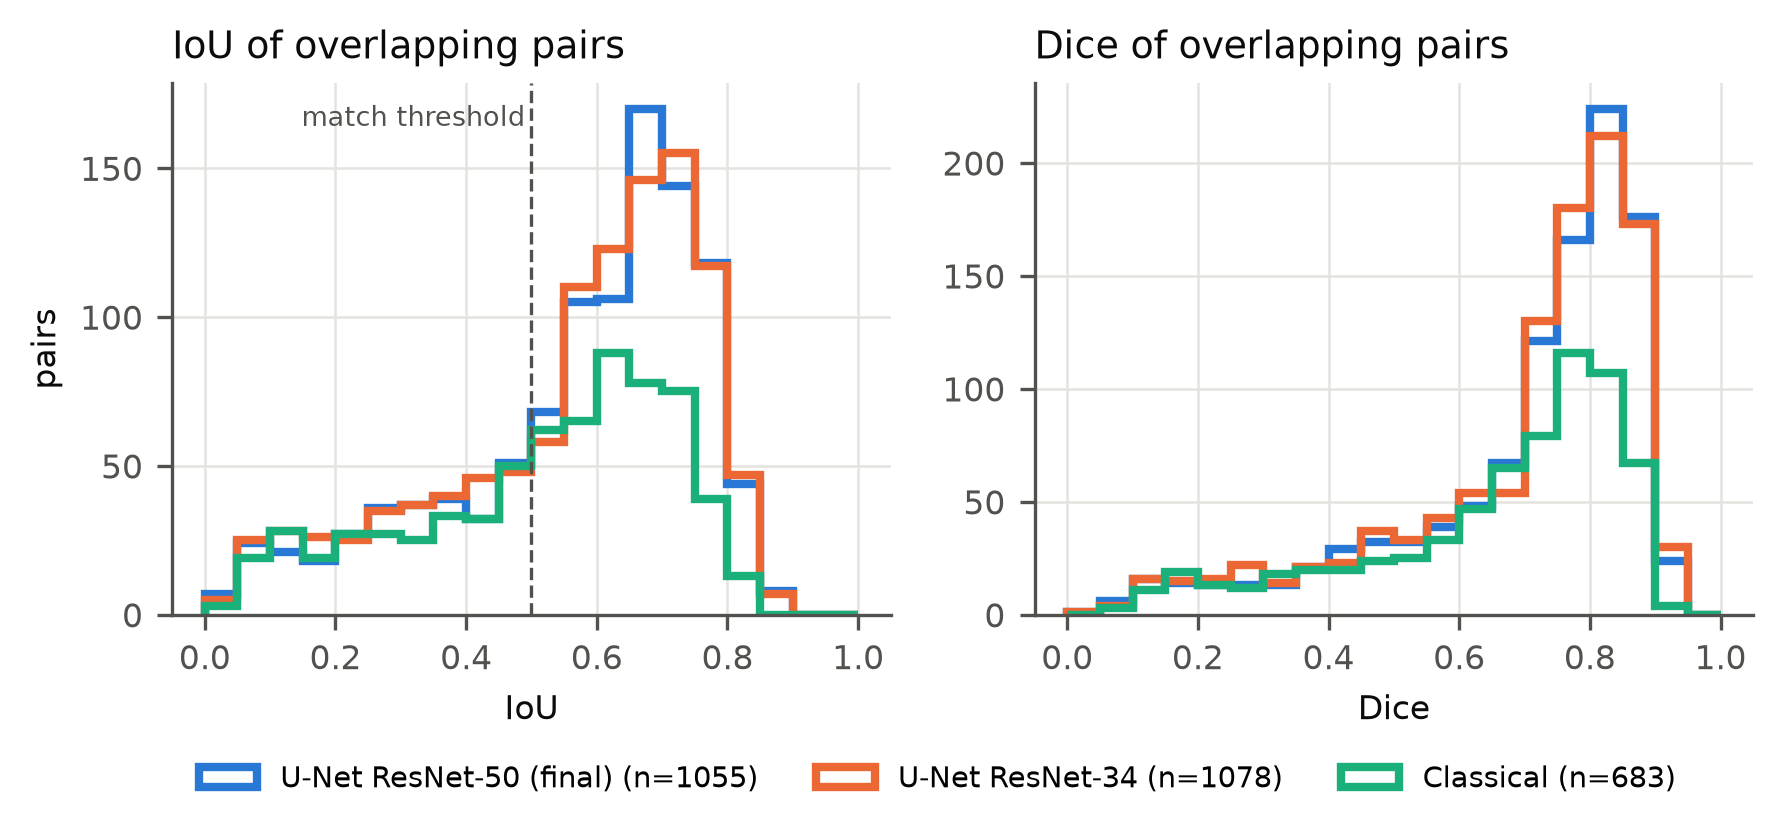
\includegraphics[width=\columnwidth]{fig_iou_dice_hist.png}
  \caption{IoU and Dice of every overlapping (annotator filament, prediction) pair on the validation set. Pairs right of the dashed line are PQ matches.}
  \label{fig:hist}
\end{figure}

\begin{figure}[t]
  \centering
  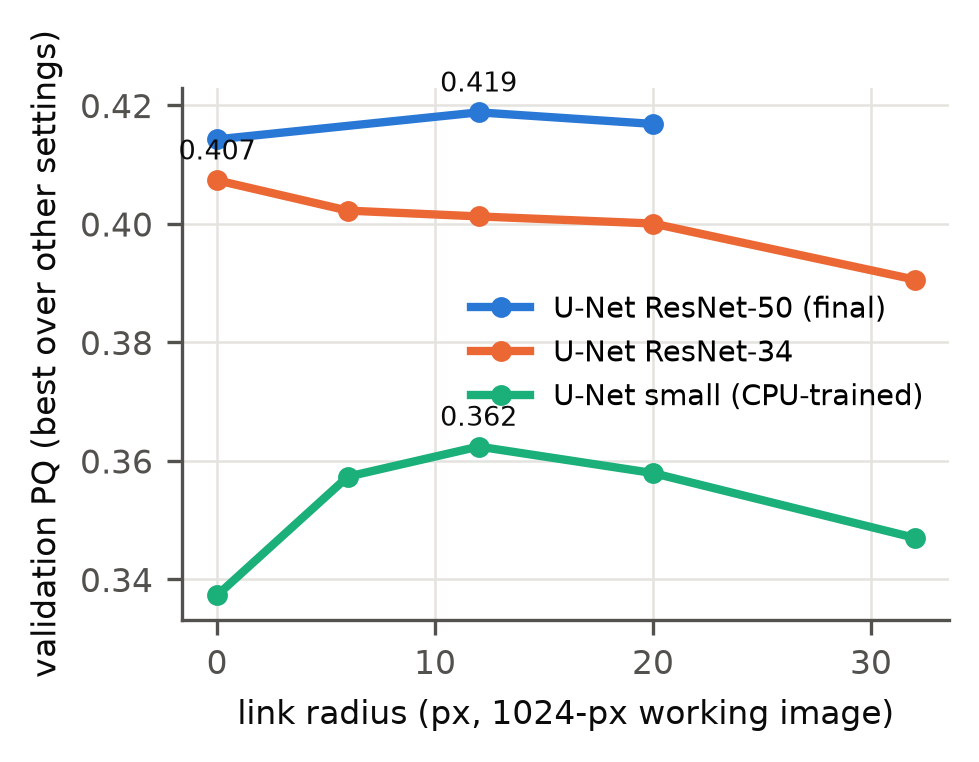
\includegraphics[width=0.8\columnwidth]{fig_pq_vs_link.png}
  \caption{Tuning PQ against the fragment link radius (best over threshold and minimum size). ResNet-50 U-Net: all 106 validation files; ResNet-34 U-Net: first 60 validation entries; compact U-Net: first 40.}
  \label{fig:link}
\end{figure}

\begin{figure}[t]
  \centering
  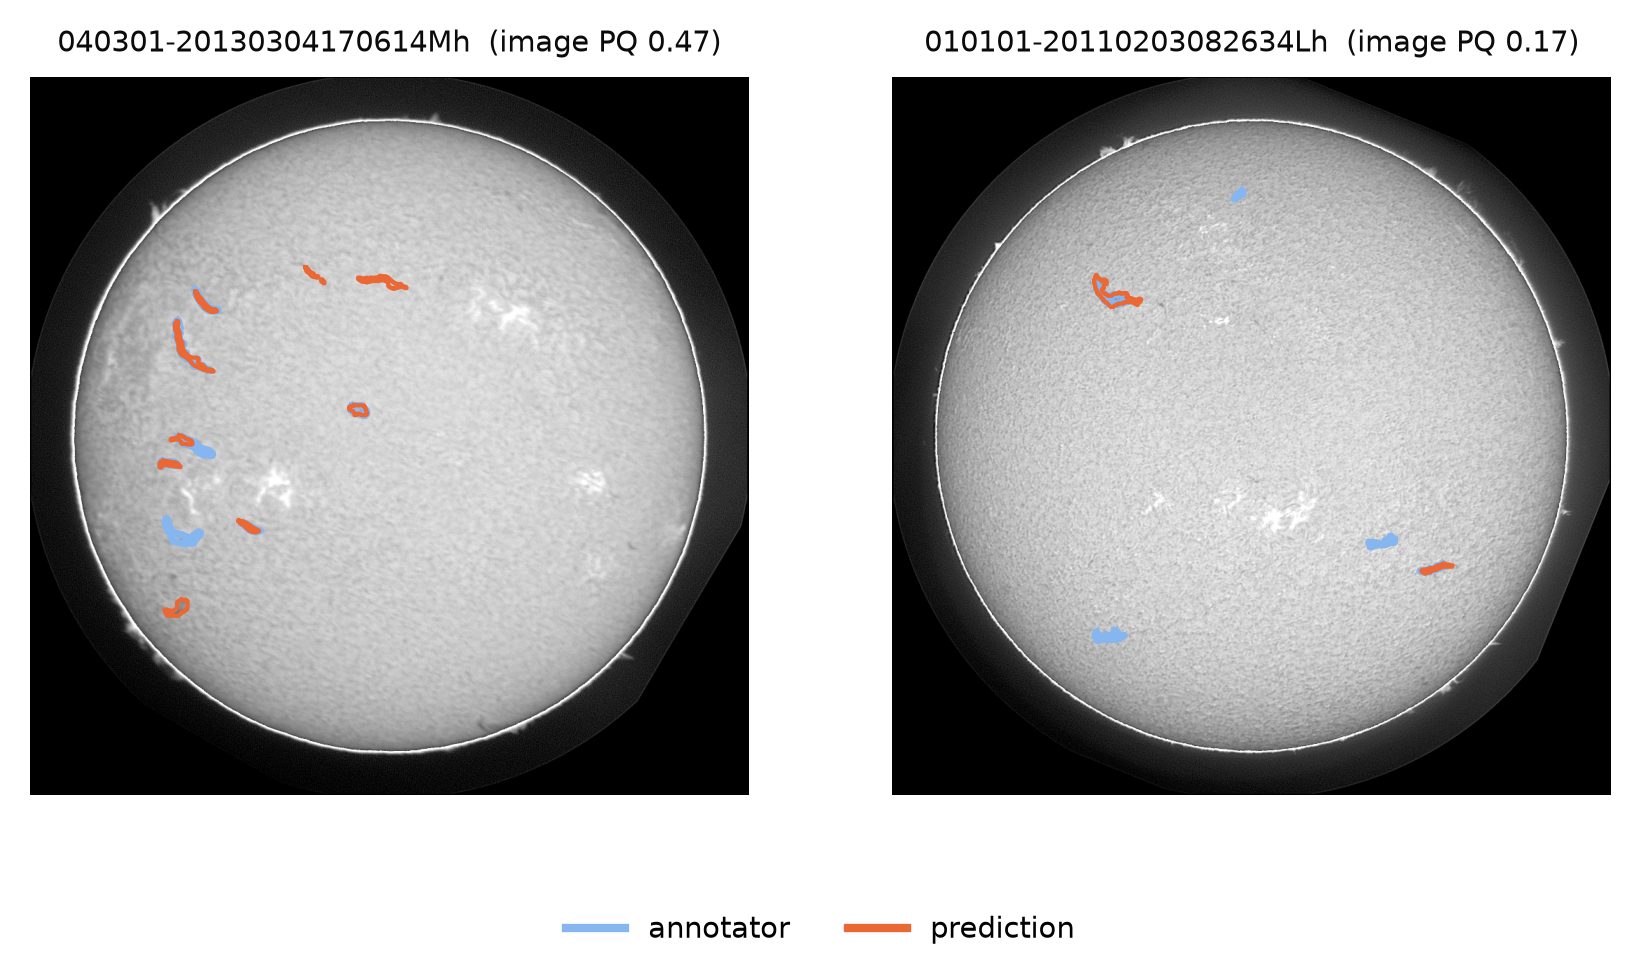
\includegraphics[width=\columnwidth]{fig_overlays.png}
  \caption{Examples: the best (left) and worst (right) of eight evenly spaced validation images. Blue: annotator; orange: prediction.}
  \label{fig:examples}
\end{figure}

\textbf{Results.} The pretrained encoder is the largest single improvement (Table~\ref{tab:results}). Compared with the compact U-Net the ResNet-34 matches 39\% more annotated filaments (763 vs 549) and misses about a third fewer (444 vs 658), raising RQ from 0.51 to 0.61, while the outline quality of the matches is similar (SQ 0.68 vs 0.67, matched Dice 0.81 vs 0.80; Fig.~\ref{fig:hist}). The deeper ResNet-50 encoder finds the same number of filaments but makes 10\% fewer false detections (493 vs 549), raising RQ to 0.62 and PQ to 0.419; scored with the same 106-file search, the ResNet-34 reaches 0.414. Flattening and PQ-based tuning are shared by all methods, so these differences come from the segmentation step. Fig.~\ref{fig:link} shows that fragment linking matters most for the weaker models: it raises the compact U-Net from PQ 0.337 ($r=0$) to 0.362 ($r=12$\,px), the ResNet-34 is almost flat up to $r=20$\,px, and the ResNet-50 gains from $r=12$\,px (0.414 to 0.419), which also lowers the one-to-many count (45 vs 70 for the ResNet-34 without linking). Averaging the probability maps of the two pretrained models (0.413), six instead of three test-time views (0.415) and simple outline shaping (dilation, smoothing, hole filling; at most +0.0002) did not help. On the public leaderboard the methods keep their validation order (0.21, 0.27, 0.33); each public score is about 0.8 times its validation PQ, so the test images appear somewhat harder but the validation set ranks the methods reliably.

\textbf{Strengths.} The pipeline needs one forward pass at 1024\,px plus two flips and runs on a laptop CPU without a GPU (15\,s per image for the ResNet-50, 6\,s for the ResNet-34); flattening makes the input consistent across sites, seeing conditions and instruments; and the post-processing is tuned for the metric that is actually judged.

\textbf{Weaknesses.} Most remaining errors are recognition errors: faint or very thin filaments are missed, and annotators disagree on which small dark features are filaments, so the same prediction can be a true positive for one annotator and a false positive for another. Thin barbs are partly lost at the 1024\,px working resolution, which lowers IoU for small filaments, and fixed-radius linking cannot separate two filaments that lie closer than $r$.

\textbf{Improvements.} Full-resolution (2048\,px) tiles, a boundary-aware loss, ensembles of models trained with different data splits, and grouping fragments along the filament spine instead of by a fixed radius.

\textbf{Reproducibility.} Code, the trained weights and \texttt{pipeline.ipynb}, which rebuilds the submission from the saved weights without retraining, are available at \url{https://github.com/amolikakkar/solar-filament-segmentation}; exact package versions are listed in \texttt{requirements.txt}. The ResNet-50 weights (130\,MB) are stored in two parts that the loader joins byte for byte. For the earlier ResNet-34 submission, the laptop-CPU notebook reproduced the GPU-produced Kaggle file exactly (all 1,475 filament masks identical), and after every code change the validation scores were re-computed and checked to be identical entry by entry.


% ==================================== %
%            ACKNOWLEDGMENT            %
% ==================================== %
\section{Acknowledgment}\label{sec:acknowledgment}
    % Do not change
    The organization of the Filament Segmentation Challenge 2026 is partially supported by the U.S. National Science Foundation (NSF) under Grant No. 2209912 and 2433781, directorate for Computer and Information Science and Engineering (CSE), and Office of Advanced Cyberinfrastructure (OAC), and Grant No. 2511630, AST Division Of Astronomical Sciences and MPS Directorate for Mathematical and Physical Sciences.

    The Filament Segmentation Challenge 2026 is sponsored by the U.S. National Science Foundation (NSF) National Solar Observatory (NSO).

    This work utilizes GONG data obtained by the NSO Integrated Synoptic Program, managed by the National Solar Observatory, which is operated by the Association of Universities for Research in Astronomy (AURA), Inc. under a cooperative agreement with the National Science Foundation and with contribution from the National Oceanic and Atmospheric Administration. The GONG network of instruments is hosted by the Big Bear Solar Observatory, High Altitude Observatory, Learmonth Solar Observatory, Udaipur Solar Observatory, Instituto de Astrofísica de Canarias, and Cerro Tololo Interamerican Observatory.

\bibliographystyle{ACM-Reference-Format}
\bibliography{main}

\end{document}
